\section{Particle storage and vectorisation}
\label{section:vectorisation}

There are three different types of data sets in our minimalistic DEM codes: 
geometric data, behavioural data and meta data. 
Behavioural data is collision data.
It is modelled as struct with location and normal vector.
Sets $\mathbb{C}$ of collision points are modelled as (dynamic) array of structs
(AoS) augmented with a copy of the collision partner as detailed before.
Spacetrees are our meta data.
The geometry data finally determines how straightforward and fast the collision
detection is---collision detection is the computationally heavy activity in the
algorithm.
While other DEM discussions speak of a computational phase \cite{xxxx}, we
prefer activity, as the collision detections are split among the grid traversal
and interwoven with other activities.


\begin{figure}
 \begin{center}
  \includegraphics[width=0.5\textwidth]{sketches/data-structure.pdf}
 \end{center}
 \caption{
   Right: The two layer data layout of our DEM code with an AoS on the particle
   level but SoA for the vector entries with replicated vector entries.
 }
 \label{figure:data-structure}
\end{figure}


We propose to realise the geometric data in two layers (Figure
\ref{figure:data-structure}).
A hull struct holds all particle properties such as velocities, rotation, mass,
geometric centre and mass centre.
Vertices refer to these hulls with arrays of structures (AoS).
Hulls link with pointers to the actual geometric data. 
This data is realised as structure of array, i.e.~there is a sequence of
x-coordinates, a sequence of y-coordinates and a sequence of z-coordinates.
These sequences are blown up with redundant data.
The first three entries in the x array hold the x coordinates of the three
vertices of the first triangle of the particle mesh.
The entries four through six hold the coordinates of the second triangle and so
forth. 
The degree of redundancy is determined by the particle mesh.


We accept the increased memory consumption of such a structure but in return are
able to avoid any indirect addressing, process all geometry data in the
collision checks in a stream-like fashion and can align all vector entries. 
SoA data are notouriously difficult to handle if subsets of a dataset are to be
transferred or data is to be reordered.
In our particle handling, a particle is an atomic unity.
It is never teared apart or resorted.
A particle mesh is topologically invariant.

The remainder of this section discusses a function \texttt{findCollisions} that
is passed two particles or two particle meshes respectively and identifies all
contact points. 
Such an operation with quadratic complexity is often wrapped into an additional
check that compares bounding boxes and thus may skip comparisons
\cite{mattutis}.
We abstain from such a check as the spacetree realises a related optimisation.
The following text thus discusses a nested loop with the outer loop
running over all triangles in $\mathbb{T}_A$ and the inner loop running over all
triangles in $\mathbb{T}_B$. 

\subsection{Brute force geometric comparison}

%
% How does the algorithm work. Robustness
%
Our default brute force approach implementation runs per triangle pair through all possible geometric
configurations (Algorithm \ref{algorithm:bf}).
Firstly, we determine the distances between each line-segment to line-segment combination (segment-to-segment stage).
Second, with all six involved vertices we compute the distance to the other triangle (point-to-triangle stage).
This yields fifteen comparisons in total. The distance between two triangles is the minimum over all computed distances.
The brute force method is a robust approach, it always yields the correct answer after the evaluation of all steps. A fusion of multiple steps is not possible because all configurations have to be evaluated naively as seen in Appendix:Algorithms \ref{algorithm:point_to_triangle}, \ref{algorithm:seg_seg}.

The calculation of distance between line segments \cite{Ericson2005} in 3D involves extending the line segments until intersection, then the closest point on the two segments is on the boundaries.
The segment $S1 = [P0, P1]$ can be formulated as $P(s) = P0+s(P1-P0) = P0+su$ with a constraint, $0<=s<=1$. Similarly, $S2 = [Q0, Q1]$
is written as $Q(t) = Q0+t(Q1-Q0) = Q0+tu$ with constraint $0<=t<=1$. So, for $sC$ and $tC$ being the closest points on the corresponding extended segments lines L1 and L2, then if  both sC and tC are within the boundaries of the segments then the closest points are also the closest points on the respective segments. 
In the case where sC and tC correspond to points on L1 and L2 outside the range of either segment $S1$ and $S2$, then sC and tC do not also define the closest points on the segments $S1$ and $S2$. So it is necessary to determine points that minimize 
$w(s,t) = P(s) - Q(t)$ over the ranges of the segments using the corresponding constraints. 
The problem can be formulated into a minimization problem where the equation w is the same as minimizing 
$|w|^2 = w \cdot w= (P0+su-tv) \cdot (Q0+su-tv)$. The relation of $|w|^2$ define a equation over a (s,t)-plane (See figure \ref{figure:ss_regions}) with a minimum at $C = (sC, tC)$, it is strictly growing along the (s,t)-plane with starting point from C. The required minimum region is not C but it is located over a subregion G of the (s,t)-plane. Using this method it is possible to perform checks to find the minimum of w(s,t) that correspond to the minimum distance between the segments.

\begin{figure}[!h]
\centering
\includegraphics[width=0.3\textwidth]{sketches/ss_box} 
\caption{(s,t) parameter space with G boundary box C for global minimum}
\label{figure:ss_regions}
\end{figure} 

The next stage of the brute force algorithm requires checking the point-to-triangle distance \ref{Eberly1999}. Using triangle T barymetic function such that $T(s, t) = B + s \cdot BA + t \cdot DA$ where $B = A$, $BA = B - A$, $DA = D - A$ for $(s,t) \in D = \{(s,t) : s \in [0,1],t \in [0,1],s + t ≤ 1\}$. The minimum distance is computed by the values $(s, t) \in D$ in distance equation $Q(s, t) = |T(s, t) - P|^2$ where $T(s,t)$ correspond to a point Q. The function can be written as: 
$Q(s,t)=as^2 +2bst+ct^2 +2ds+2et+f$ where $a = BA \cdot BA$, $b = BA \cdot DA$, $c = D-A \cdot DA$, $d = B-A \cdot (B - P)$, $e = DA \cdot (B - P)$, and $f = (B - P) \cdot (B - P)$. So for function Q, $ac - b2$ = $(B-A \cdot B-A)(E1 \cdot D) - (B-A \cdot B-A)^2$ =$|B-A \cdot D-A|^2 >0$. The positivity is based on the assumption that the two edges $B-A$, $D-A$ are linearly independent. The minimum occurs at an interior point of D where the gradient $\nabla Q = 2(as + bt + d, bs + ct + e) = (0, 0)$ or at a point on the boundary of D. The gradient of Q is zero only when $s = (be - cd)/(ac - b^2)$ and $t = (bd - ae)/(ac - b^2).$  If $(s,t) \in D$ (See Figure \ref{figure:pt_regions}) then minimum of Q is found. 

\begin{figure}[!h]
\centering
\includegraphics[width=0.4\textwidth]{sketches/pt_regions} 
\caption{Regions based on the (s,t) parameters plane}
\label{figure:pt_regions}
\end{figure}

On the other hand if the minimum is not in D then it is on the boundary of the triangle. Using the active constraints we restrict the solution so if (s, t) is in region one then the level curves of Q are constant. As the level value V increase from $V_{min}$ as they growing away from $(s,t)$ there is a smallest level value that is tangent to the  domain $D$ with $s+t = 1$. So for any level values $V < V_{min}$, the corresponding do not intersect $D$. However for any portion of $D$ that intersect levels V must be $V > V_{min}$. Therefore in this case point $(s0, t0)$ provides the minimum distance between P and the triangle where $t0$ is known $t0 = 1 - s0$ and $s0$ is the only unknown to be solved. Moreover, when minimization is happening at $\nabla Q(s, 1 − s) = 0$ then there are three cases where $s > 1$ and $s$ has to be restricted to $s=1$ and the minimum occurs at $\nabla Q(1, 0)$ because of the constraints. Similarly if $s < 0$ then minimum occurs when $\nabla Q(0,1)$ or lastly $s \in [0,1]$. Similarly the same technique for determining whether the minimum occurs at the endpoints or at the interior interval of the corresponding constraints is performed for all regions.


\subsection{Penalty-based formalism}

\begin{algorithm}
	\protect\caption{\label{alg4}MATLAB Penalty Solver.}
	\begin{algorithmic}[1]
	\Function{Penalty}{A, B, C, D, E, F, rho, tol}

		\State $BA~=~B-A;~CA~=~C-A;~ED~=~E-D;~FD~=~F-D;$

		\State $hf~=~{[}2{*}BA{*}BA',~2{*}CA{*}BA',-2{*}ED{*}BA',-2{*}FD{*}BA';$

		\State $2{*}BA{*}CA',~2{*}CA{*}CA',-2{*}ED{*}CA',-2{*}FD{*}CA';$

		\State $2{*}BA{*}ED',-2{*}CA{*}ED',~2{*}ED{*}ED',~2{*}FD{*}ED';$

		\State $2{*}BA{*}FD',-2{*}CA{*}FD',~2{*}ED{*}FD',~2{*}FD{*}FD'{]};$

		\State $x~=~{[}0.33;~0.33;~0.33;~0.33{]};$

		\For{i=1:99}

			\State $X~=~A+BA{*}x(1)~+~CA{*}x(2);$

			\State $Y~=~D+ED{*}x(3)~+~FD{*}x(4);$

			\State $gf~=~{[}2{*}(X-Y){*}BA';~2{*}(X-Y){*}CA';~-2{*}(X-Y){*}ED';~-2{*}(X-Y){*}FD'{]};$

			\State $h~=~{[}-x(1);~-x(2);~x(1)+x(2)-1;~-x(3);~-x(4);~x(3)+x(4)-1{]};$

			\State $dh~=~{[}-1,~0,~1,~0,~0,~0;~0,~-1,~1,~0,~0,~0;$

			\State $0,~0,~0,~-1,~0,~1;~0,~0,~0,~0,~-1,~1{]};$

			\State $mask~=~h'~$>$=~0;$

			\State $dmax~=~dh.{*}~{[}mask;~mask;~mask;~mask{]};$

			\State $gra~=~gf~+~rho~{*}~dmax~{*}~max(0,h(:));$

			\State $hes~=~hf~+~rho{*}dmax{*}dmax'~+~eye(4,4)/rho^2;$

			\State $dx~=~hes\textbackslash{}gra;$

			\State $DX~=~BA{*}dx(1)~+~CA{*}dx(2);$

			\State $DY~=~ED{*}dx(3)~+~FD{*}dx(4);$

			\State $error~=~sqrt(DX{*}DX'+DY{*}DY');$

			\If{error~$<$~tol}
				\State $BREAK;$
			\EndIf

			\State $x~=~x~-~dx;$

		\EndFor

	\EndFunction
	\end{algorithmic}

\end{algorithm}
\subsection{Hybrid approach}
To create a hybrid solver we first assume that on average there are for each triangle pair distance computation only a few iterations that are required to arrive to a solution \ref{}. Based on empirical studies and tuning of the penalty parameter and the regularization variable, the majority of triangle pairs are solved within four iterations as shown in Figure {}. Secondly we set a user defined tolerance of error to the method to act as the switching point for the falling-back to brute force solver. If the number of fall backs does not overtake the number of penalty-based solutions then the method is a compromise between brute force and penalty both in terms of performance but also in terms of error of solution. 

\begin{figure}[htb]
  \begin{center}
    \includegraphics[width=1\textwidth]{experiments/random/penalty-stats/bar.png}
  \end{center}
  \caption{Histogram of number of iterations required by Newton Method for convergence on a sample of twenty four million triangle pair configurations.}
  \label{figure:newton_hist}
\end{figure}

There are two variants of hybrid method; the first is the hybrid-on-triangle-pairs and the second one is hybrid-on-triangle-batches. Both variants are developed to exploit the robustness of brute force while keeping the arithmetic intensity of the penalty method. The implementation of both methods takes into account the potential for shared memory scaling as well as data access continuity. In addition SIMD vectorised performance of the underlying methods and memory alignment are critical for the execution of both methods.

The first variant is hybrid-on-triangle-pairs where it divides the computational workload to be per each triangle pair. The hybrid-on-triangle-pairs method runs first the penalty solver on one triangle pair, if the solution is not within the user specified tolerance, we fall back to brute force to solve the problem naively. 

\begin{algorithm}
 \caption{Hybrid On Triangle Pairs} \label{algorithm:hybridTriangle}
 \begin{algorithmic}[1]

	\Function {hybridOnTrianglePairs(particleA, particleB, tolerance)}	
	
		\For {i = 0 to n particleA.triangles}
	
			\For {j = 0 to n particleB.triangles}
			
				\State {triangleError = penalty(particleA[i], particleB[j])}

				\If {triangleError > tolerance}

					\State {bruteForce(particleA[i], particleB[j])}
	
				\EndIf
	
			\EndFor
			
		\EndFor
		
		\Return {P, Q points on two triangles}
	
	\EndFunction
	
 \end{algorithmic}
\end{algorithm} 

The other variant is the hybrid-on-batches where it is hybrid per triangle batches. This method is checking the error less frequently than the previous variant and uses an error for the whole batch. As in the hybrid-on-triangle-pairs variant; we run then penalty method on one batch of triangles and then fall back to brute on the whole batch if the error tolerance is not satisfied. The batch size can be set by the user to be of any arbitrary size. For our application we set it to be the number of triangles of our non-spherical particles (tessellation size of 60~ triangles).    

\begin{algorithm}
 \caption{Hybrid On Triangle Batches} \label{algorithm:hybridBatches}
 \begin{algorithmic}[1]
	
	\Function {hybridOnTrianglePairs(particleA, particleB, tolerance)}	
	
		\For {i = 0 to n particleA.triangles}
	
			\For {j = 0 to n particleB.triangles (batchSize)}
					
				\State {batchError = penalty(particleA[i], particleB[j])}

			\EndFor
			
			\If {batchError > tolerance}
				
				\For {j = 0 to n particleB.triangles}
	
					\State {bruteForce(particleA[i], particleB[j])}

				\EndFor
	
			\EndIf
	
		\EndFor
	
		\Return {P, Q points on two triangles}	
	
	\EndFunction
	
 \end{algorithmic}
\end{algorithm} 

Both hybrid methods suffer by their nature by the granularity of the grain size whether that is singular size (triangle pair) or greater (batches of pairs).
The memory distribution of pairs of triangles that do not converge within the mean number of Newton iterations are not known a priori because the solution depends on the underlying geometry. Triangle pairs or triangle batches that do not converge within the set tolerance skew the overall error distribution margin, potentially creating the worse case scenario where the method becomes a worse than brute force solver with both penalty and brute force being executed in sequence. It is not possible to predict the sparsity/distribution of non-convergent triangle pairs/batches during run-time so the tolerance value, penalty, regularization parameters are vital. In our experiments those parameters are set based on empirical tuning and trial and error.


